\section{M2M Communications architecture}
\label{sec:overveiw-ref-m2m-arch}
% I intend to present key elements in M2M system, especially in cellular network.
% 其实关于M2M architecture的原则则是至今都在讨论的东西。。。
% 参考: System improvement for Machine-Type Communications
Given that there is not a consensus about MTC reference architecture, standardization developing organizations (SDO) and research community have proposed a few of proposals. ETSI provides a general M2M reference architecture with purpose of designing an access and transmission technology independent service middle layer~\cite{ETSI/TS/102/690}. Nowadays the architecture-related works are transferred to oneM2M. The project oneM2M published their reference architecture at the beginning of 2015, which is similar but different than that of ETSI M2M. 3GPP proposes a MTC reference architecture with focus on improvement of core network~\cite{3GPP/TR/23888V11}. 
IEEE 802.16p gives an overall architecture for M2M~\cite{IEEE-requirement-doc}. 
The authors of~\cite{Loa2013} review and compare the aforementioned architectures then propose a hybrid reference model. Since the reference architectures of 3GPP and IEEE 802.16p are functionally equivalent, mainly the efforts of ETSI, oneM2M and 3GPP are presented. 
\subsection{ETSI M2M reference architecture}
The ETSI proposes a high level reference architecture for M2M communication, which is illustrated in Fig.~\ref{fig:etsi-ref-arch} and composed by a device-and-gateway domain and a network domain~\cite{ETSI/TS/102/690}. This architecture consists of the following components: \begin{itemize}[leftmargin=*, noitemsep]
	\item M2M-D, a device running M2M applications usually embedded in a smart device and replies to requests or sends data;
	\item M2M area network, a capillary network (e.g. small-scale home environment) composed by individual M2M-D leveraging short-range communication technologies  (e.g. IEEE 802.15.1, Zigbee, Bluetooth, etc.)
	\item M2M-G, a proxy responsible for interworking for M2M area network and Network domain.
	\item Access Network, a network that provides access to the core network for devices (i.e. M2M-D and M2M-G) in device-and-gateway domain. It can be, among others, in form of the access network of 3GPP, xDSL, satellite and WiMAX.
	\item Core Network, a network that provides various services such as IP connectivity, network control, interworking, roaming and so on between M2M-A and M2M-D. It includes, but is not limited to, 3GPP CN, ETSI TISPAN CN and 3GPP2 CN.
	%从 a cellular-centric service architecture 文中摘得,注意改写描述避免抄袭问题
	\item M2M-A, M2M Applications, application services that run the service logic and use M2M-SC via application programming interfaces.
	\item M2M-SC, a network node providing M2M functions to M2M-A and hiding network specificities for M2M application development.
\end{itemize}
\begin{figure}[!t]
	\centering
	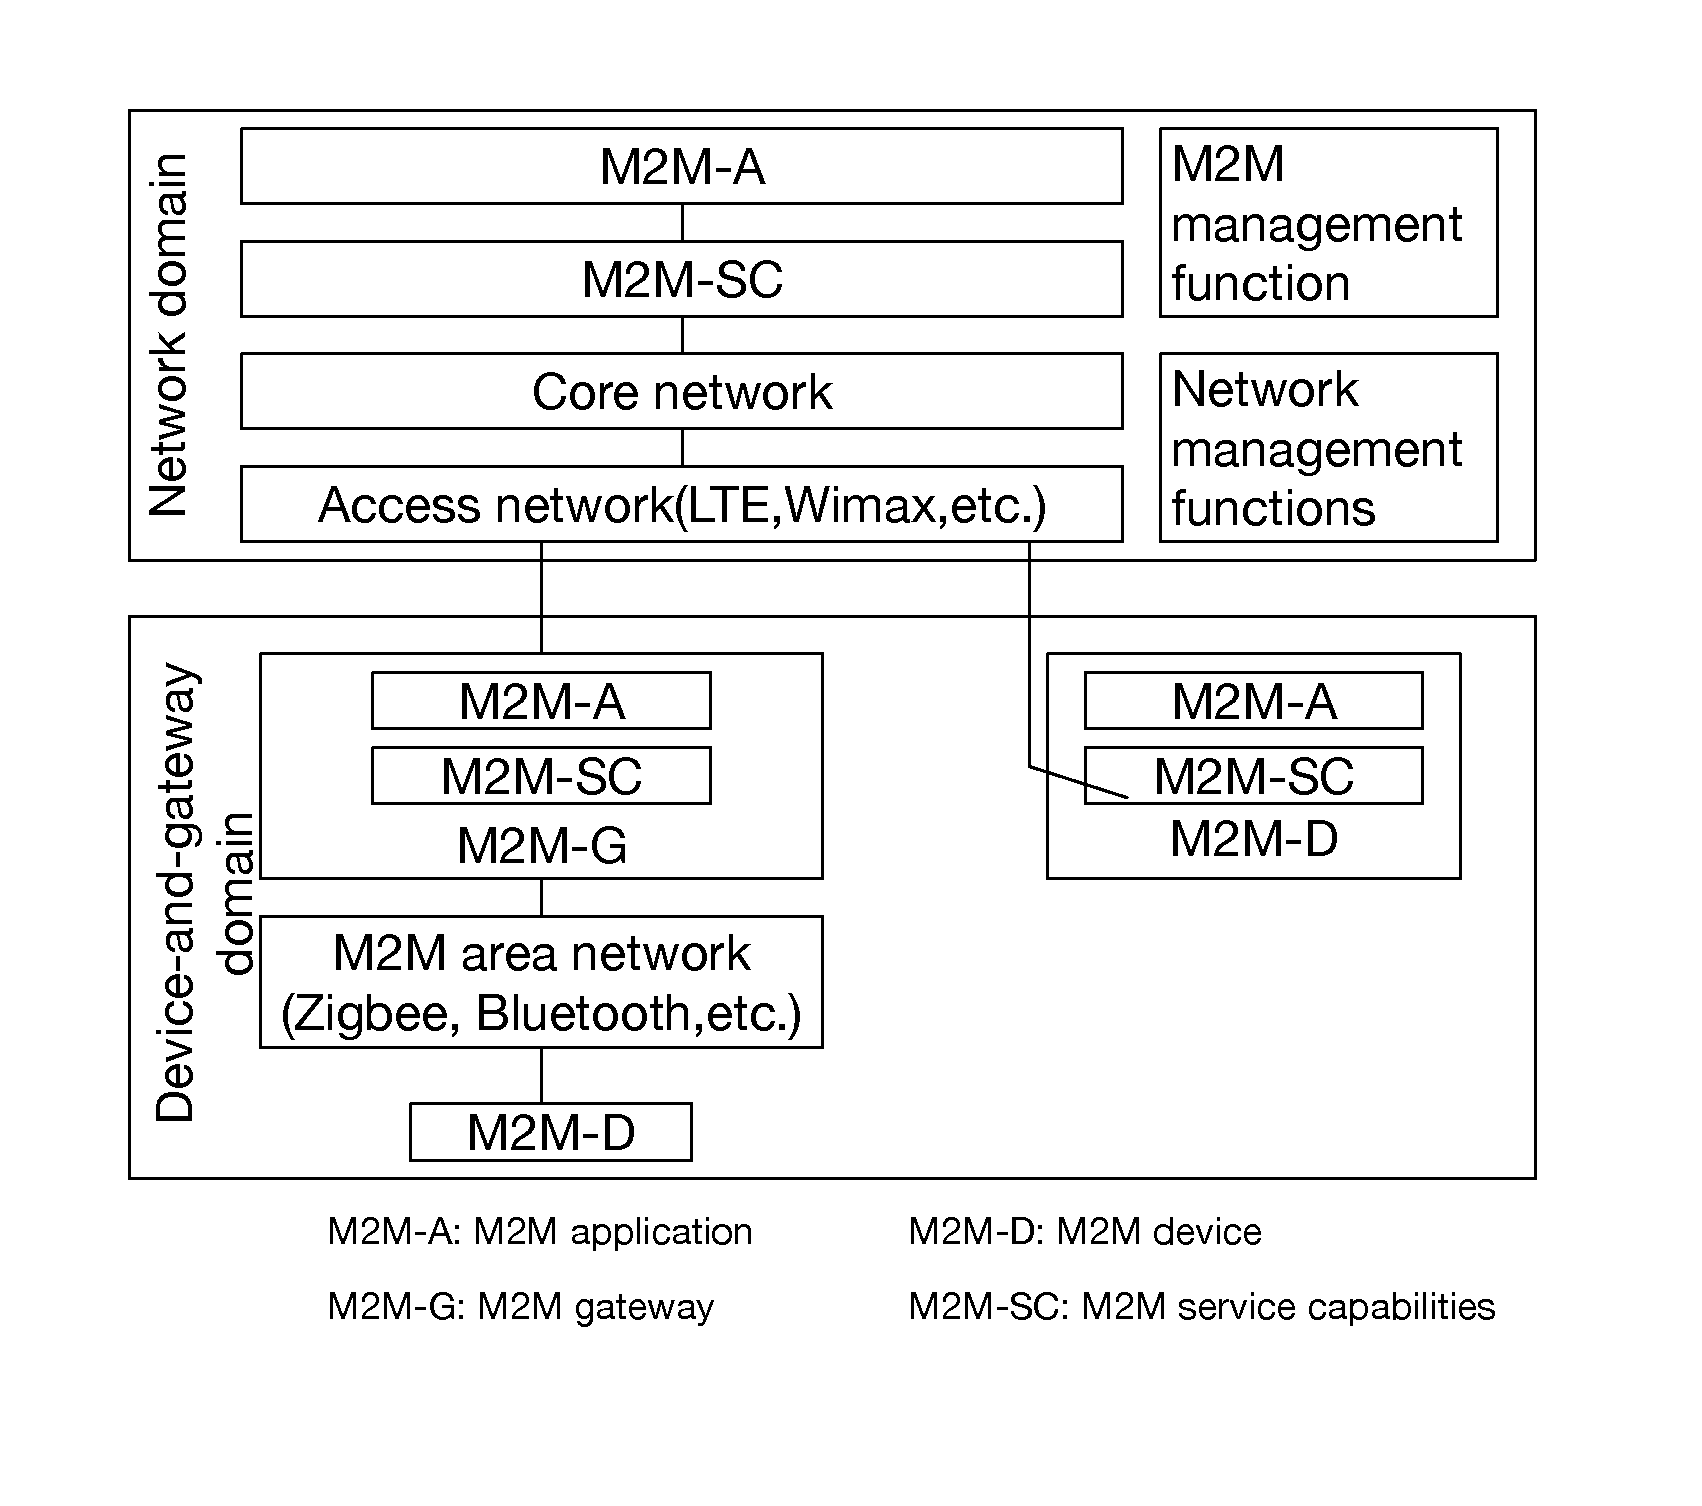
\includegraphics[width=0.8\linewidth]{Chapter2/Figures/ETSI-ref-architecture}
	\caption{ETSI reference M2M communication architecture. (Modified based on~\cite{ETSI/TS/102/690})}
	\label{fig:etsi-ref-arch}
\end{figure}
\subsection{oneM2M reference architecture}
% 部分信息提取自网络资源:http://www.etsi.org/plugtests/COAP2/Presentations/03_ETSI_M2M_oneM2M.pdf
% https://ec.europa.eu/research/innovation-union/pdf/active-healthy-ageing/arndt.pdf
% https://www.afnic.fr/medias/documents/JCSA/2014/05-Arndt-ETSI-M2M-and-oneM2M-JCSA-2014.pdf
Apart from the efforts of ETSI M2M, other regional SDOs conduct standardization activities. To avoid the risks of divergence,  the oneM2M partnership project was established in 2012 by leading regional SDOs such as ETSI (Europe), TIA and ATIS (North America), CCSA (China), TTA (Korea), ARIB and TTC (Japan). The objective of oneM2M is to prepare, approve and maintain globally applicable, access-independent technical specifications and reports related to M2M solutions, with initial focus on the Service Layer. The functional architecture of oneM2M is shown in Fig.~\ref{fig:onem2m-ref-arch}. There exist mainly three functions: Application Entity (AE), Common Services Entity (CSE) and Network Services Entity (NSE). Application Entity is an entity in the application layer that implements an M2M application service logic and equivalent to the M2M-A in ETSI reference architecture (shown in Fig.~\ref{fig:etsi-ref-arch}). The Common Services Entity represents an instantiation of a set of \emph{common service function} (i.e. M2M service
subscription management,  device management, etc.)
A Network Services Entity hides the implementation of underlying communication networks and  provides services to the CSEs. The oneM2M reference architecture reuses principles and solutions from ETSI M2M: the entity AE is like the M2M-A in Fig.~\ref{fig:etsi-ref-arch}. The CSE is equivalent to the M2M-SC in Fig.~\ref{fig:etsi-ref-arch}. The infrastructure is similar to the ETSI network domain and the field domain is like the device and gateway domain of ETSI.
\begin{figure}[!t]
	\centering
	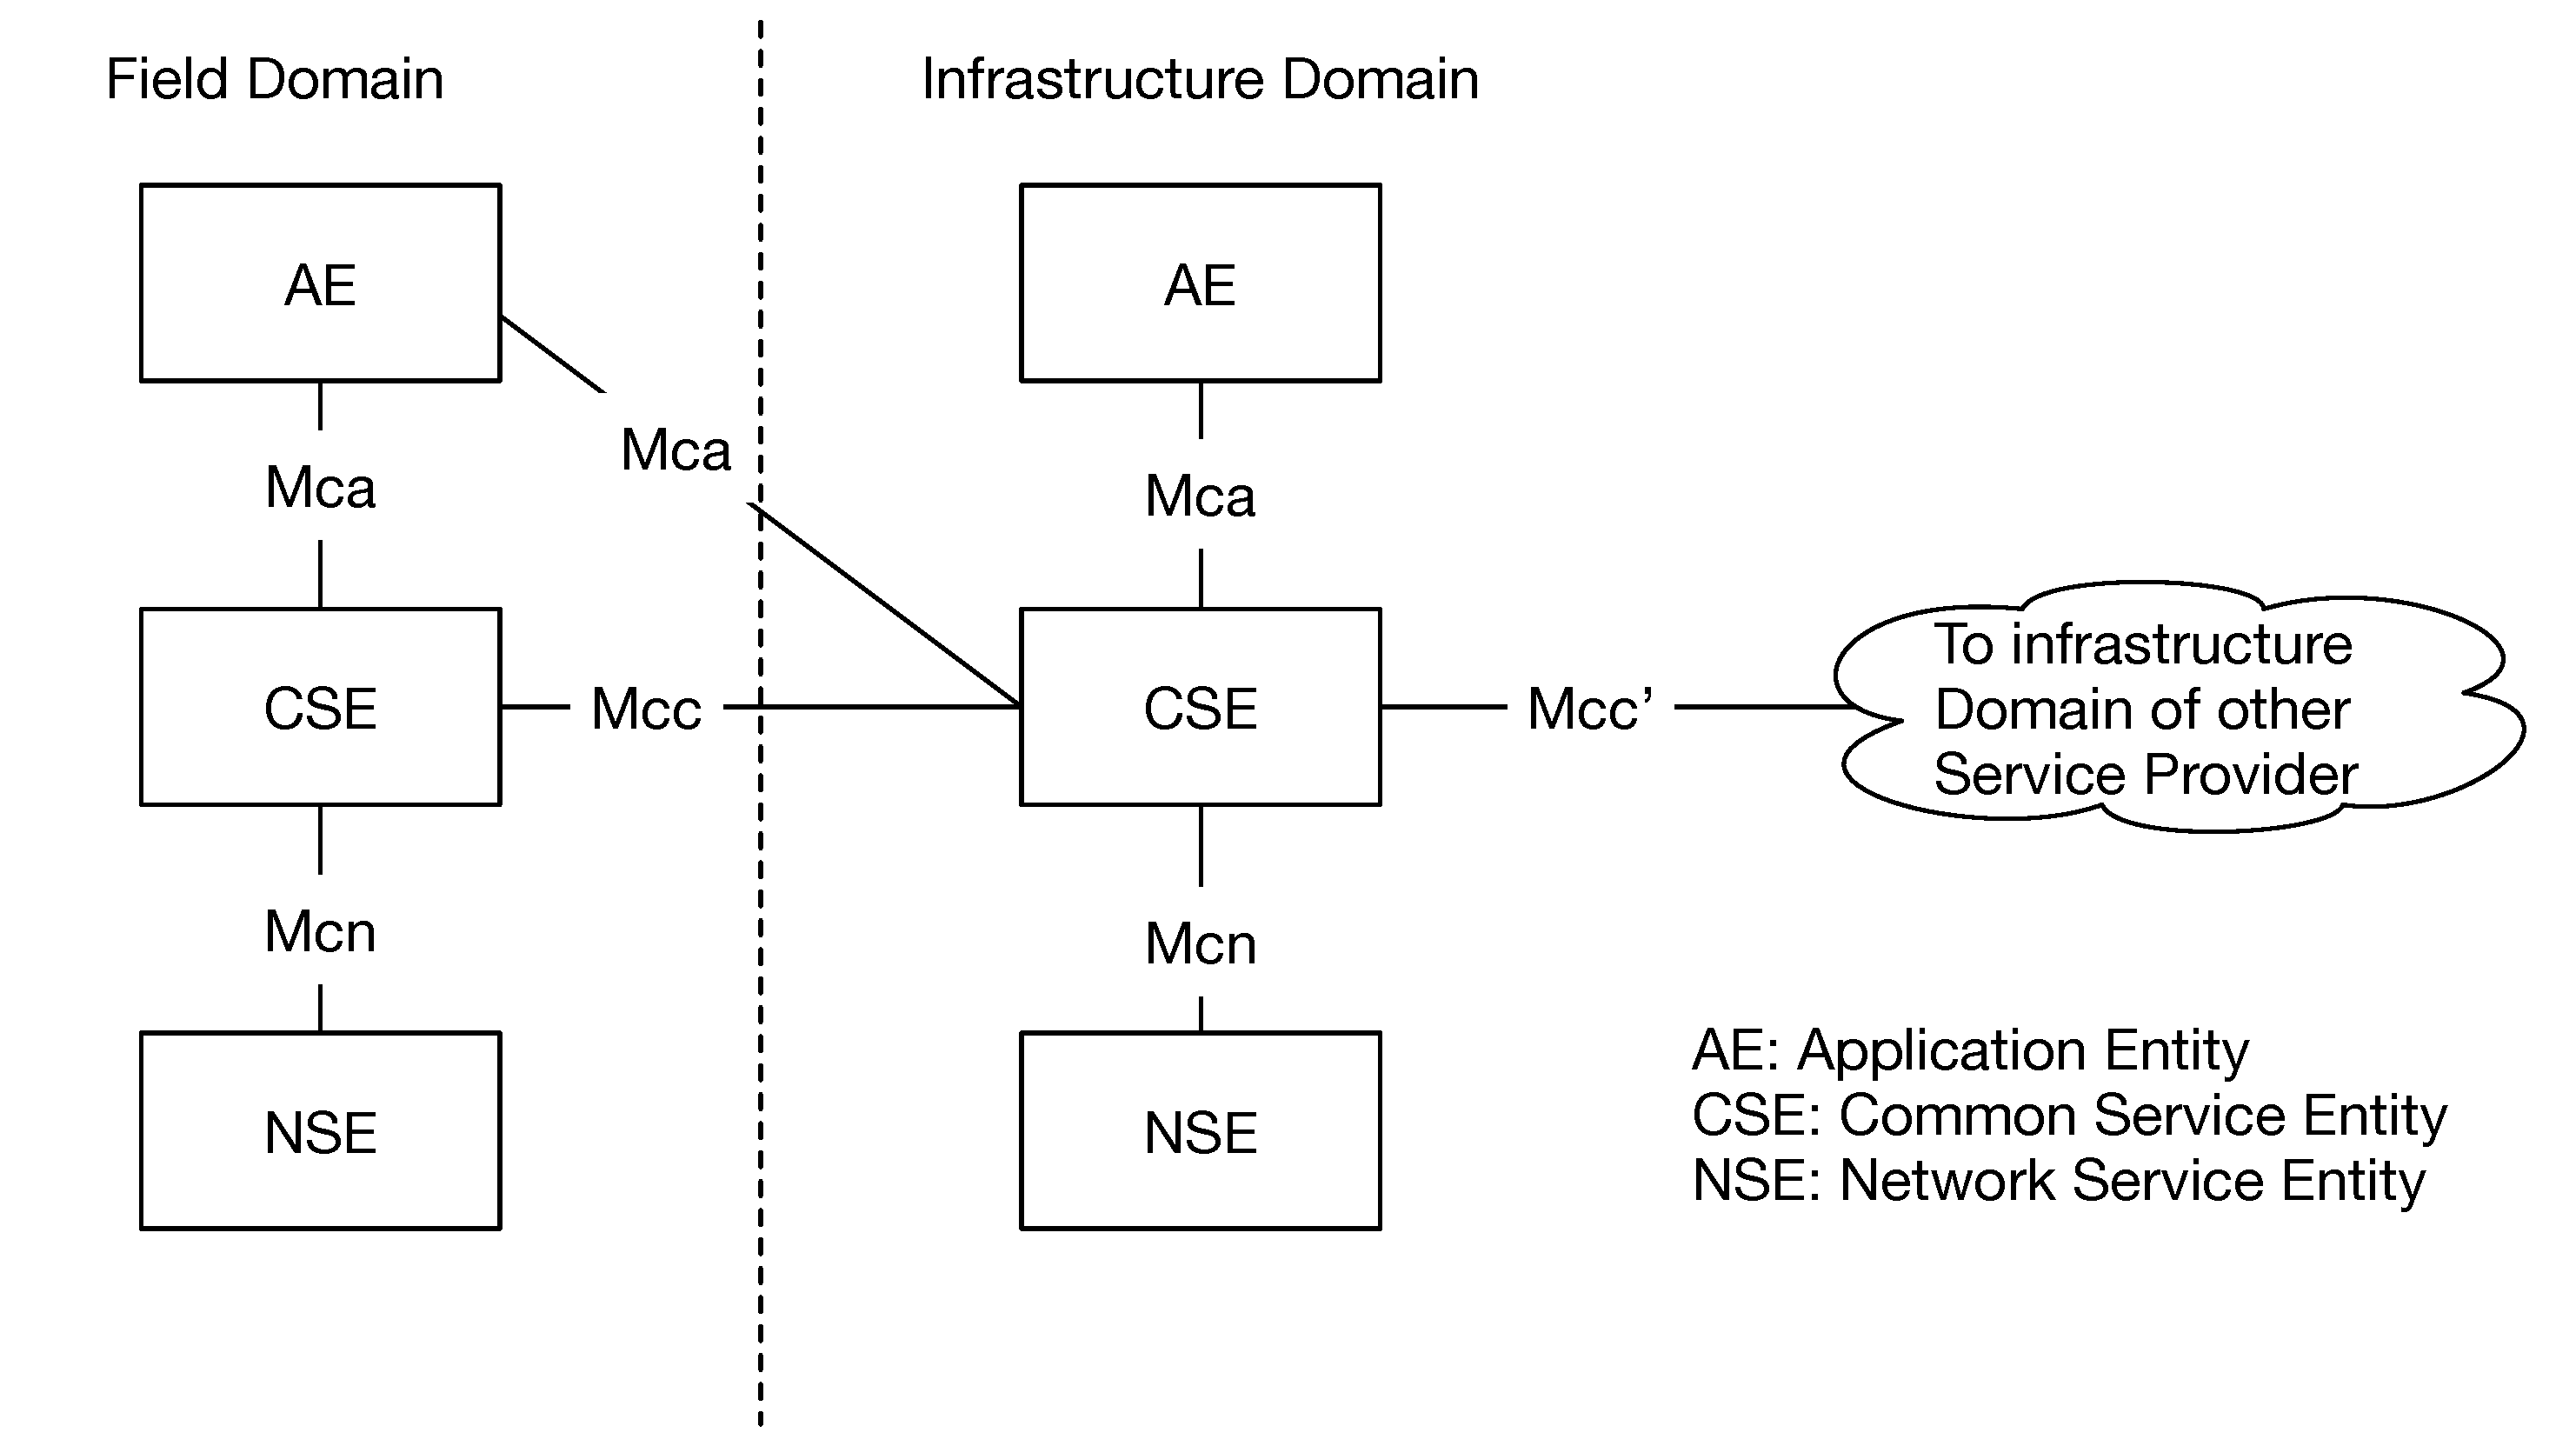
\includegraphics[width=0.8\linewidth]{Chapter2/Figures/oneM2M-reference-architecture}
	\caption{oneM2M reference functional M2M architecture. Source: \cite{onem2m/funcarch}}
	\label{fig:onem2m-ref-arch}
\end{figure}
\subsection{3GPP reference MTC architecture}
The main contribution of ETSI M2M overall architecture is to standardize the resource structure representing the information contained in M2M-SC, but ETSI has not specified the standardization for M2M area network, access network and core network.
% 3GPP 2012-09 在 System improvement 提过一个 reference model
% 同年11月又在 Architecture enhancement to facilitate communicateions with...中 提出了一个新的改进型 architecture, 并引入了 SCS 的概念
The efforts of 3GPP about MTC architecture are summarized in~\cite{3GPP/TS/23682}\cite{3GPP/TR/23888V11}. Different from that of ETSI, the focuses of 3GPP are mainly cellular wireless network, especially the access and core network. The proposed reference architecture is shown in Fig.~\ref{fig:3gpp-ref-arch}.
\begin{figure}[!t]
	\centering
	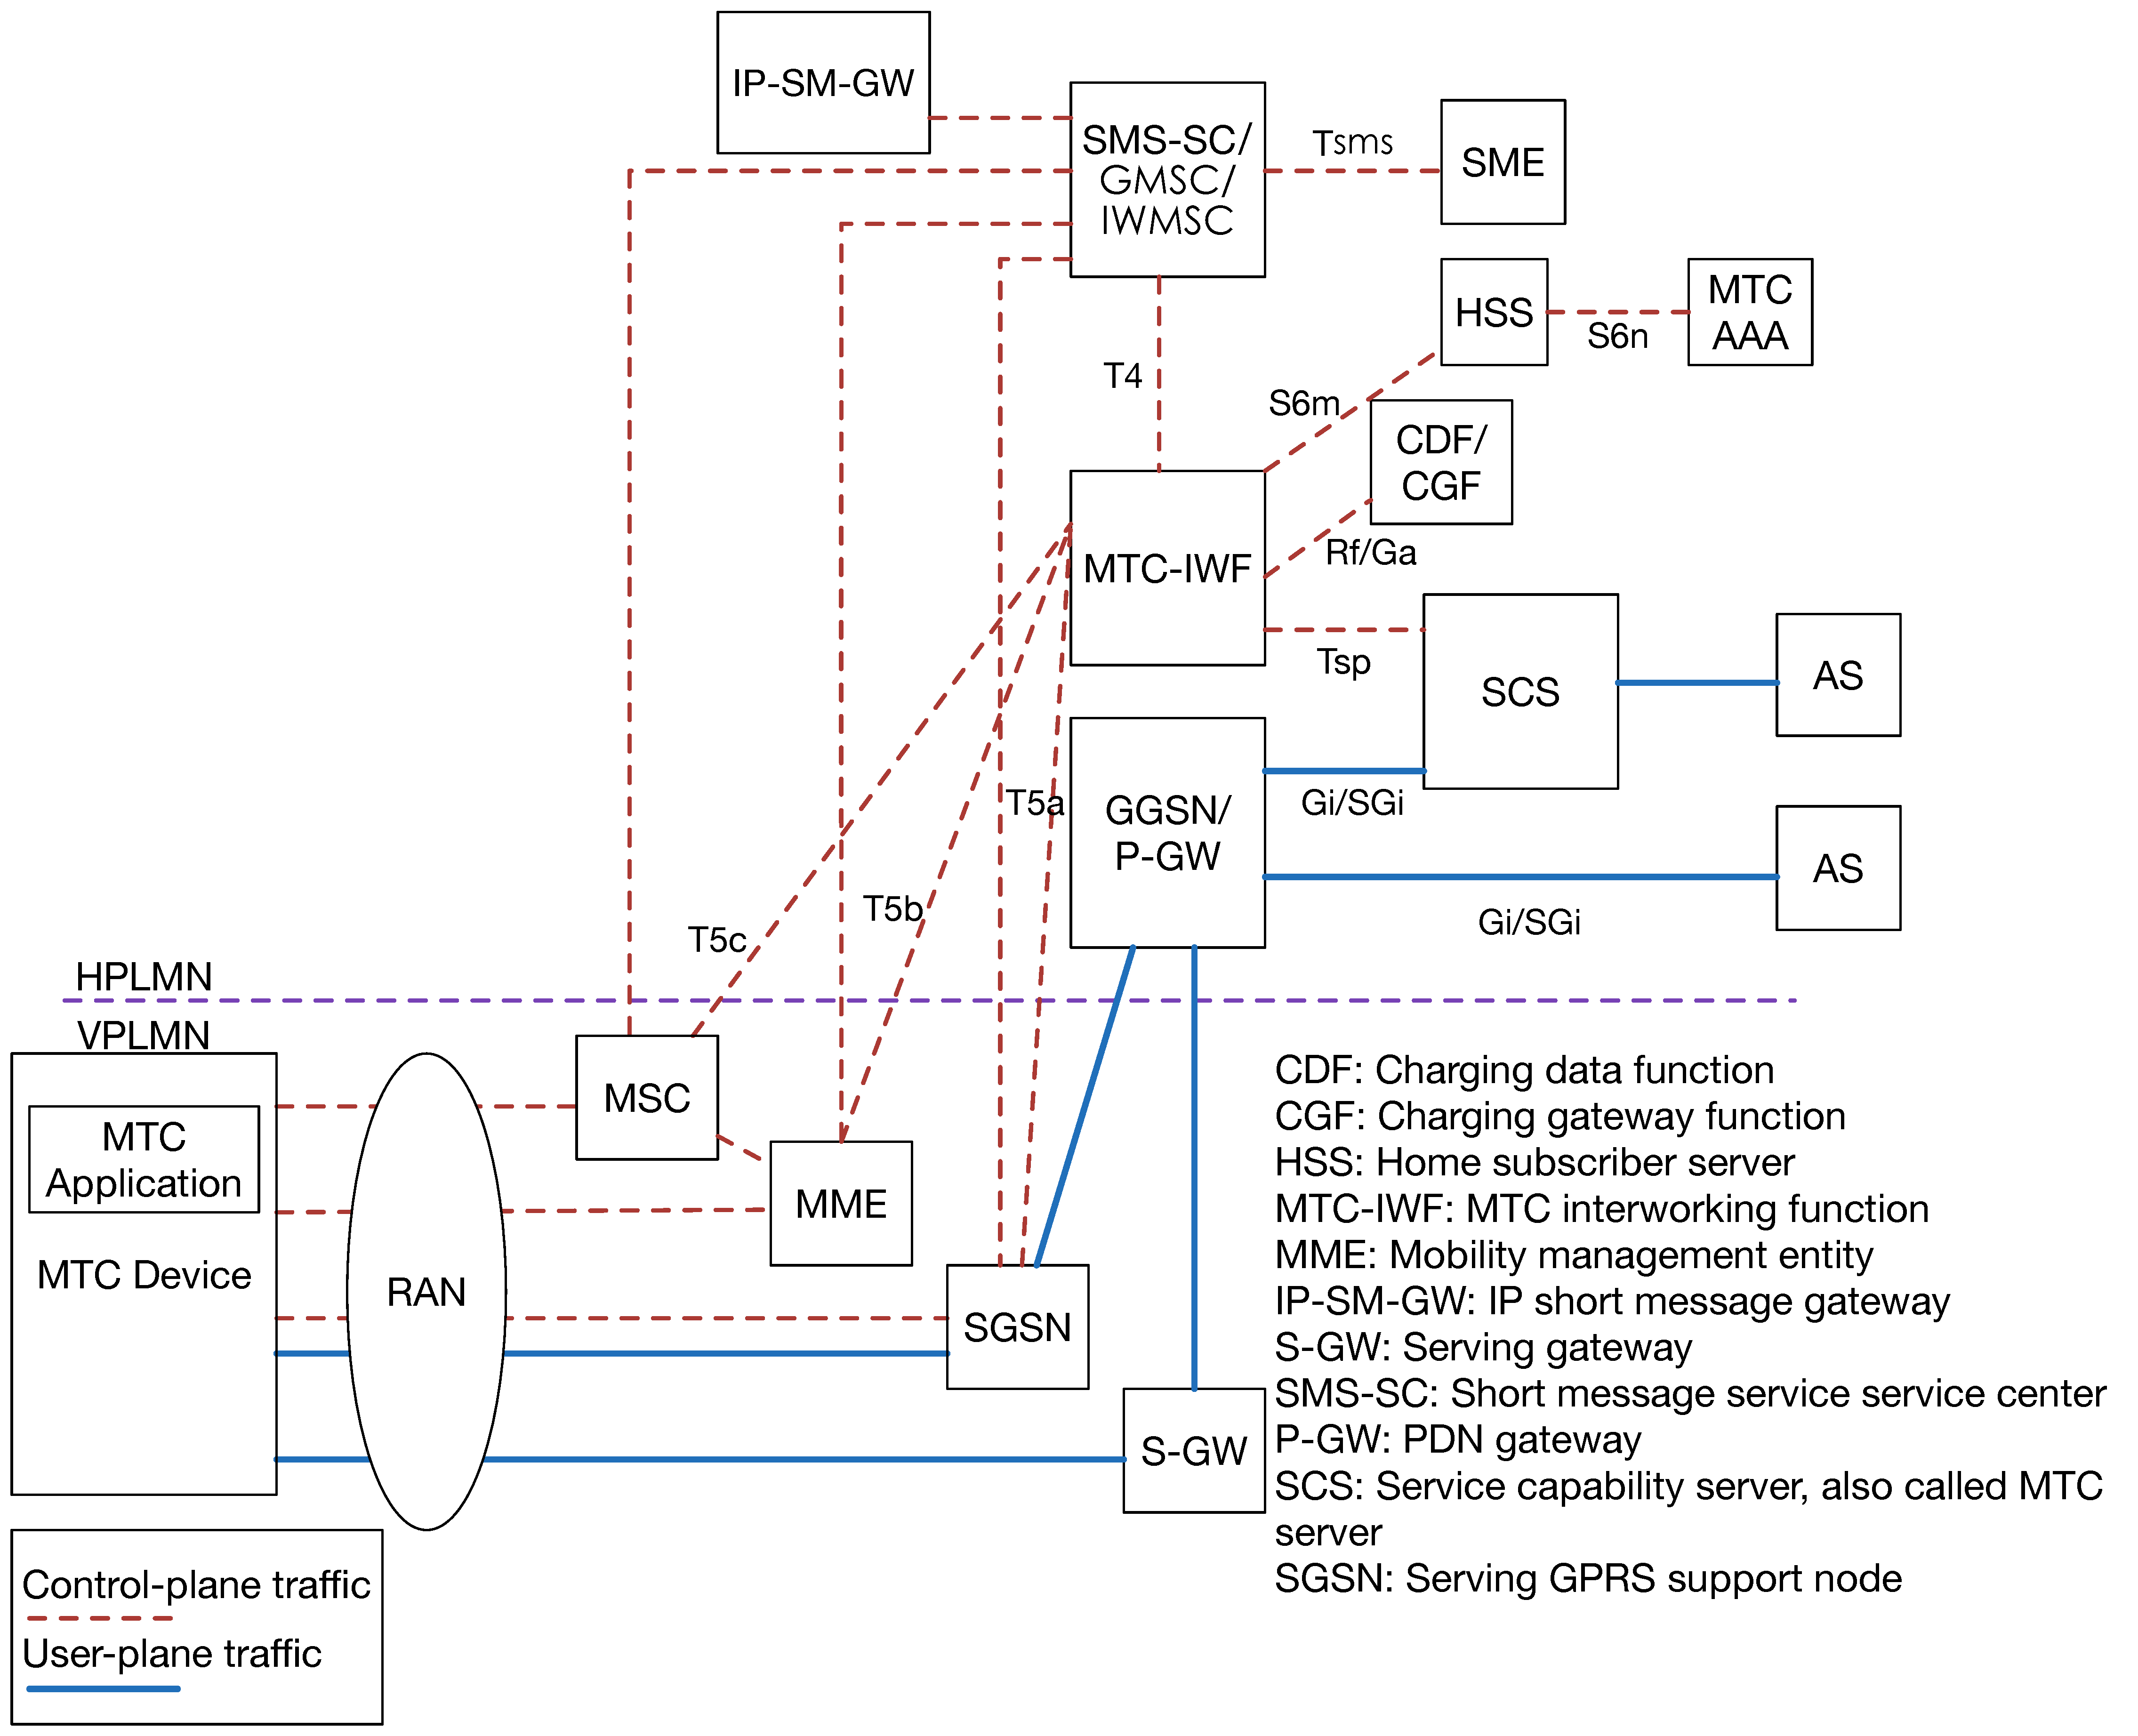
\includegraphics[width=0.9\linewidth]{Chapter2/Figures/3GPP-ref-architecture-V2}
	\caption{3GPP reference MTC architecture. (based on \cite{3GPP/TR/23888V11} )}
	\label{fig:3gpp-ref-arch}
\end{figure}
The enhancement made by 3GPP supports the device trigger function. To this end, two new network nodes (MTC-IWF and SCS) and a series of reference points related to these two nodes are introduced. The first node, MTC Interworking function (MTC-IWF), hides the internal PLMN (Public Land Mobile Network) topology and relays or translates signaling protocols used over Tsp (shown in Fig.~\ref{fig:3gpp-ref-arch}) to invoke specific functionality in the PLMN. The main functions of MTC-IWF are: to authorize the SCS before communication establishment with the 3GPP network, receive a device trigger request from SCS, select the most efficient and effective device trigger delivery mechanism, etc.
%以下内容直接摘自 3GPP: Architecture enhancements to facilitate communications with packet data networks and applications
The SCS is an entity that connects to the 3GPP network to communicate with MTC devices and the MTC-IWF in the HPLMN. This entity offers capabilities to be used by one or multiple MTC Applications, and is controlled either by the mobile operator or a MTC Service Provider. 

\subsection{M2M architecture in the literature}
Combining the respective advantages of proposals of 3GPP and ETSI, Lo et al. propose a cellular-centric M2M service architecture based on LTE-A specification~\cite{Loa2013}, which is shown in Fig.~\ref{fig:hybrid-ref-arch}. Their proposal is a four-tier architecture:
\begin{itemize}[leftmargin=*, noitemsep]
	\item Tier 1: The tier 1 consists of M2M applications and servers (namely M2M-A and M2M-S).
	\item Tier 2: The most distinguished change is at tier 2, in which a new functional entity M2M-R (M2M relay function) is introduced.  M2M-R is an extension of the conventional LTE-A relay functionality. This extension enables LTE-A relay node to act as a M2M data concentrator.
	\item Tier 3: The most important functional entity at tier 3 is M2M-G, which is actually a gateway to serve M2M devices non 3GPP-compliant. The full-fledged 3GPP MTC-G implementation has not been standardized ant thus is still an open research issue.
	\item Tier 4: The tier 4 consists of those non 3GPP-compliant M2M devices (e.g., devices using ZigBee, etc.)
\end{itemize}
The proposal in~\cite{Loa2013} actually leverages M2M gateway (M2M-R) to support non 3GPP compliant devices. The introduction of the M2M-R aggregates the packets from a large number of M2M devices into a single large packet, adds system capacity and then reduces transmission.
\begin{figure}[!t]
	\centering
	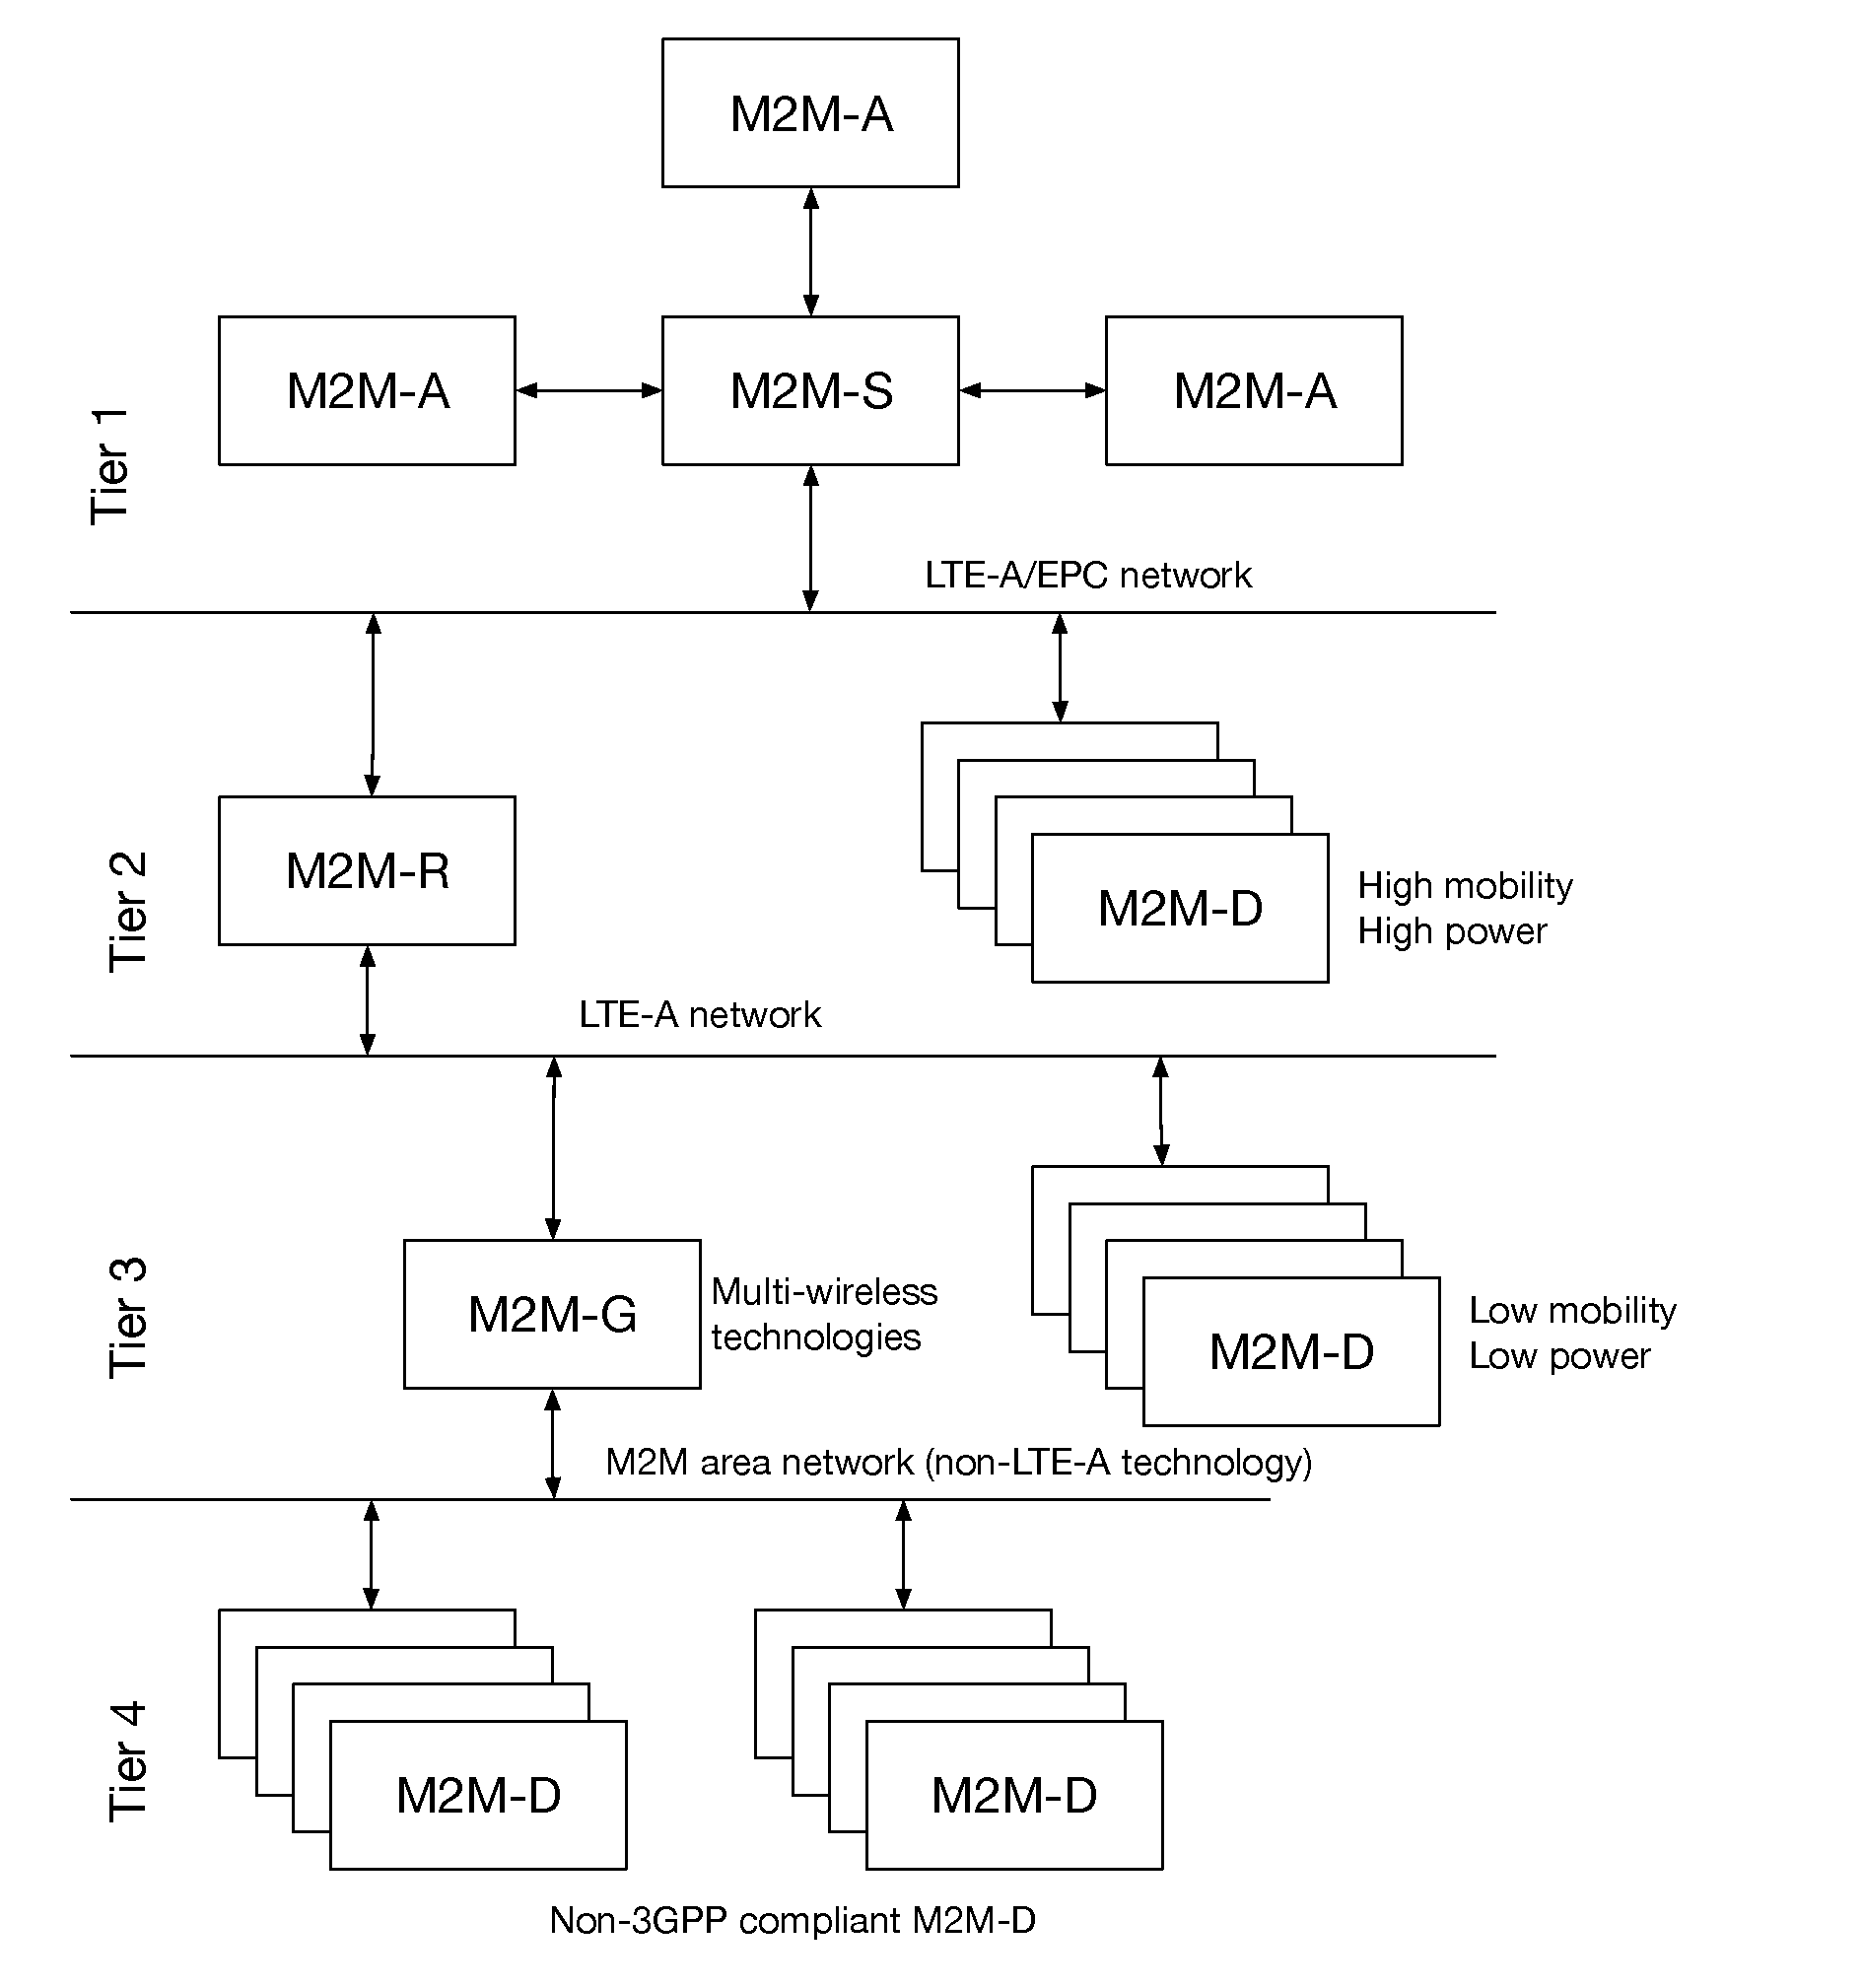
\includegraphics[width=0.95\linewidth]{Chapter2/Figures/Hierarchical-LTE-A-cellular-centric-M2M-service-architecture}
	\caption{Hierarchical-LTE-A-cellular-centric-M2M-service-architecture. Source: \cite{Loa2013}}
	\label{fig:hybrid-ref-arch}
\end{figure}